\documentclass[first=dblue,second=red,logo=blueexc]{aaltoslides}
%\documentclass{aaltoslides} % DEFAULT
%\documentclass[first=purple,second=lgreen,logo=redque,normaltitle,nofoot]{aaltoslides} % SOME OPTION EXAMPLES

\usepackage[utf8]{inputenc}
\usepackage{graphicx}
\usepackage{amssymb,amsmath}
\usepackage{url}
\usepackage{caption}
\usepackage{subcaption}
\usepackage{lastpage}
\usepackage{array}
\usepackage{booktabs}   
\usepackage{pbox}
\usepackage{multicol}
\usepackage{multirow}

\title{Twitter the Rioter :\\Analyzing roles through a protest on social media.\\ \emph{\large What was your part during the 2014 Ferguson riots?}}

\author[J. Blégean]{Julien Blégean}
\institute[ICS]{Degree Programme in Computer Science and Engineering\\
Aalto University, School of Science and Technology\\julien.blegean@aalto.fi}

\aaltofootertext{Example Slides}{\today}{\arabic{page}/\pageref{LastPage}\ }

\setbeamertemplate{section in toc}[circle]

\date{Version 1.0, \today}

\begin{document}

%%%%%%%%%%%%%%%%%%%%%%%%%%%%%%%%%%%%%%%%%%%%%%%%%%%%%%%%%%%%%%%%%%%%%%%%%%%%%%%%%%%%%%%%%%%%%

\aaltotitleframe

%%%%%%%%%%%%%%%%%%%%%%%%%%%%%%%%%%%%%%%%%%%%%%%%%%%%%%%%%%%%%%%%%%%%%%%%%%%%%%%%%%%%%%%%%%%%%

\begin{frame}{Introduction}
\begin{itemize}

\item 2011 : London riots, Arab spring
\begin{itemize}
\item first use of the social medias for protests
\item UK government about to shut down Facebook \& Twitter
\item \textbf{topic of interest}
\end{itemize}

\item 2014 : Ferguson riots
\begin{itemize}
\item Twitter again blamed
\item interesting dataset because :
\begin{itemize}
\item English content (US)
\item recent
\item the US use Twitter a lot
\end{itemize}
\end{itemize}

\item \textbf{Focus on the roles}

\begin{itemize}
\item how to model it?
\item how to find similar users ?
\item how to visualize it?
\end{itemize}

\end{itemize}
\end{frame}

%%%%%%%%%%%%%%%%%%%%%%%%%%%%%%%%%%%%%%%%%%%%%%%%%%%%%%%%%%%%%%%%%%%%%%%%%%%%%%%%%%%%%%%%%%%%%

\begin{frame}{Outline}
\tableofcontents
\end{frame}

%%%%%%%%%%%%%%%%%%%%%%%%%%%%%%%%%%%%%%%%%%%%%%%%%%%%%%%%%%%%%%%%%%%%%%%%%%%%%%%%%%%%%%%%%%%%%

\section{Dataset structure and basic analysis}
\begin{frame}{Outline}
\tableofcontents[sectionstyle=show/shaded]
\end{frame}

%%%%%%%%%%%%%%%%%%%%%%%%%%%%%%%%%%%%%%%%%%%%%%%%%%%%%%%%%%%%%%%%%%%%%%%%%%%%%%%%%%%%%%%%%%%%%

\begin{frame}{Dataset}
\begin{itemize}
\item $\sim$ 12 million tweets
\item August 11 - August 27
\end{itemize}

\end{frame}

%%%%%%%%%%%%%%%%%%%%%%%%%%%%%%%%%%%%%%%%%%%%%%%%%%%%%%%%%%%%%%%%%%%%%%%%%%%%%%%%%%%%%%%%%%%%%

\begin{frame}{Dataset}
\framesubtitle{Structure of a tweet}

\begin{figure}[h!]
\centering
\begin{tabular}{ccc}
field & type & example\\
\hline
\hline
id & number & \texttt{498619822134280192} \\ \hline
publication date & date & \texttt{2014-08-11 00:00:04} \\ \hline
author id & number & \texttt{124010717} \\ \hline
text & number & \pbox{5cm}{\vspace*{5pt}\texttt{Please follow @AntonioFrench now! \newline \#Ferguson \#MikeBrown http://t.co/---}\vspace*{5pt}} \\ \hline
retweet count & number & \texttt{4} \\ \hline
is it a retweet ? & boolean & \texttt{False} \\ \hline
hashtags & string list & \texttt{\#Ferguson, \#MikeBrown} \\ \hline
links and medias & string list & \texttt{http://t.co/---} \\ \hline \hline
\end{tabular}
\end{figure}

\end{frame}

%%%%%%%%%%%%%%%%%%%%%%%%%%%%%%%%%%%%%%%%%%%%%%%%%%%%%%%%%%%%%%%%%%%%%%%%%%%%%%%%%%%%%%%%%%%%%

\begin{frame}{Dataset}
\framesubtitle{Structure of a user}

\begin{figure}[h!]
\centering
\begin{tabular}{ccc}
field & type & example\\
\hline
\hline
user id & number & \texttt{14090948} \\ \hline
name & string & \texttt{Antonio French} \\ \hline
nickname & string & \texttt{AntonioFrench} \\ \hline
registration date & date & \texttt{2008-03-06 19:51:29} \\ \hline
tweet count & number & \texttt{19372} \\ \hline
followers count & number & \texttt{119977} \\ \hline
friends count & number & \texttt{1373} \\ \hline \hline
\end{tabular}
\end{figure}


\end{frame}

%%%%%%%%%%%%%%%%%%%%%%%%%%%%%%%%%%%%%%%%%%%%%%%%%%%%%%%%%%%%%%%%%%%%%%%%%%%%%%%%%%%%%%%%%%%%%

\begin{frame}{Frequencies}

\begin{figure}[h!]
\begin{center}
	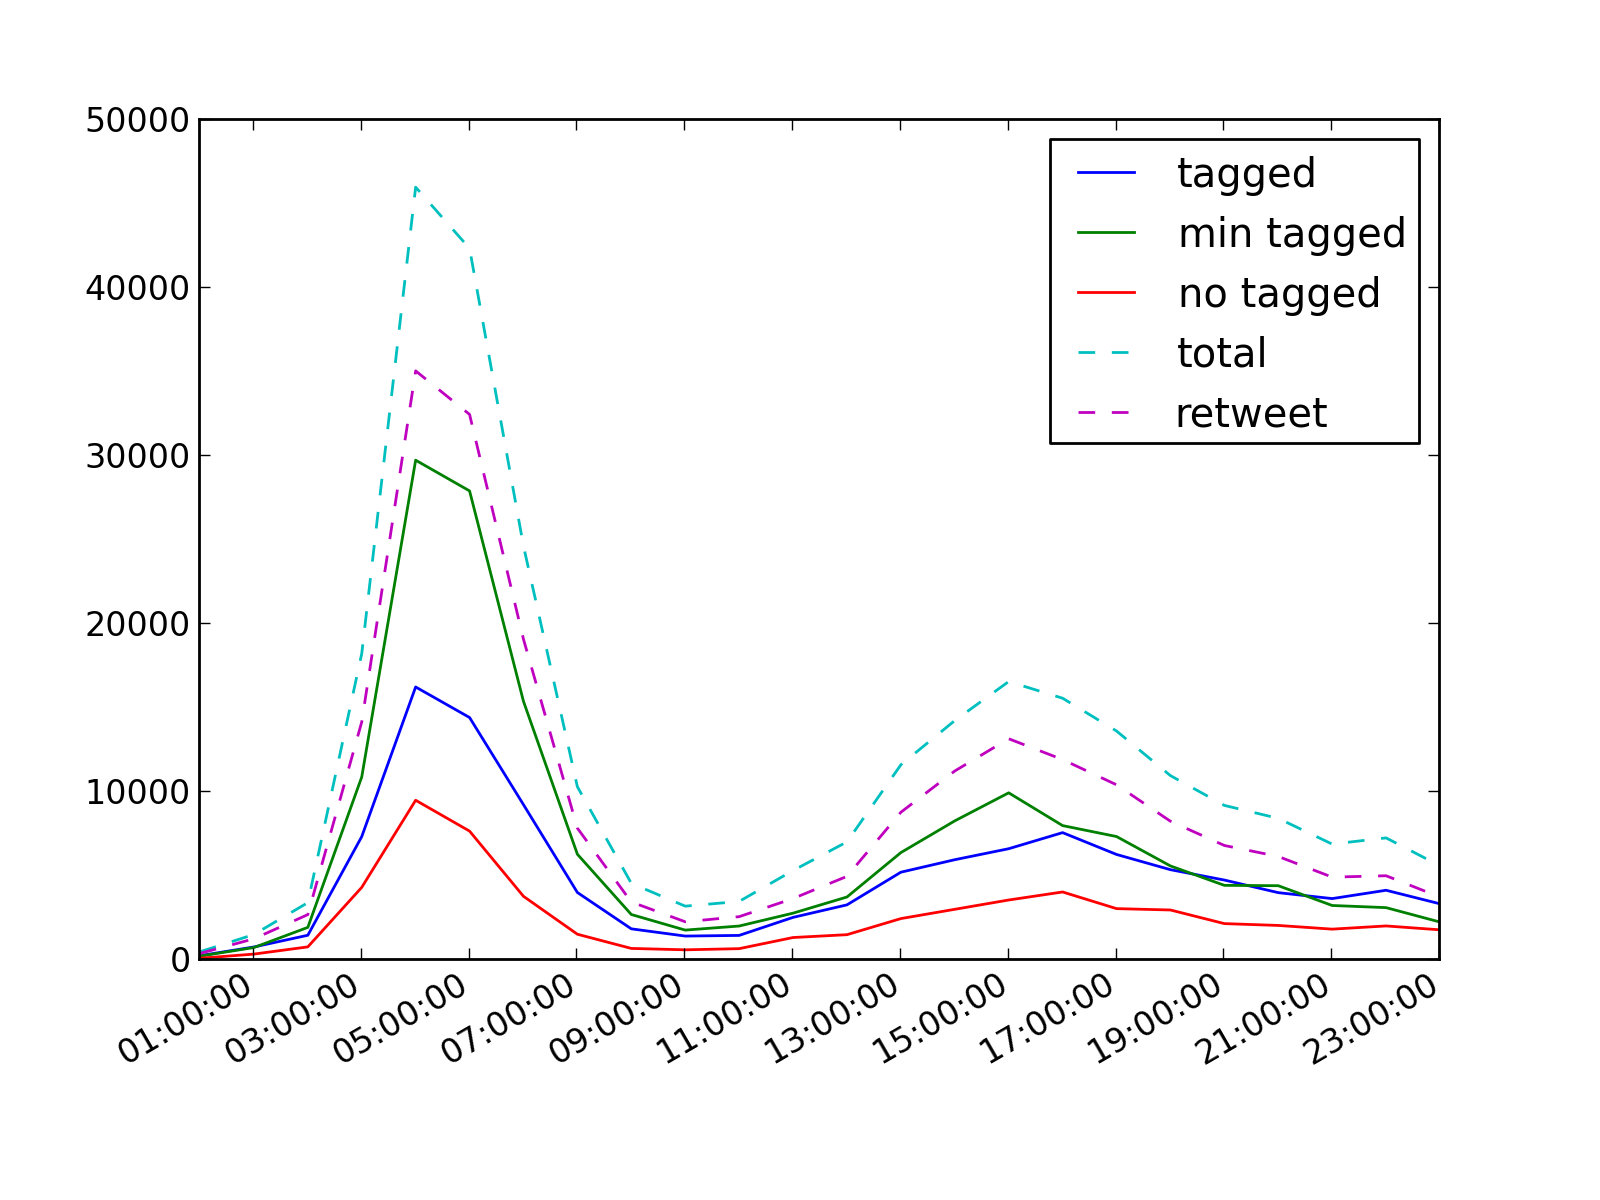
\includegraphics[width=0.7\textwidth]{images/freqs/freq_11_08.png}
	\caption{August 11th}
\end{center}
\end{figure}


\end{frame}

%%%%%%%%%%%%%%%%%%%%%%%%%%%%%%%%%%%%%%%%%%%%%%%%%%%%%%%%%%%%%%%%%%%%%%%%%%%%%%%%%%%%%%%%%%%%%

\section{Clustering tweets : finding topics}
\begin{frame}{Outline}
\tableofcontents[sectionstyle=show/shaded]
\end{frame}

\begin{frame}{Tweet embedding}
\begin{itemize}
\item $\text{Vocabulary} = \{\text{word} | \text{word in top $n$} \}$
\item Tweet embedding \\
\[
\bordermatrix{
~ & word_1 & word_2 & \cdots & word_n \cr 
tweet_1 & tfidf_{1,1} & tfidf_{1,2} & \cdots & tfidf_{1,n} \cr
tweet_2 & tfidf_{2,1} & tfidf_{2,2} & \cdots & tfidf_{2,n} \cr
\hspace{12pt}\vdots & \vdots & \vdots & \ddots & \vdots \cr
tweet_m & tfidf_{m,1} & tfidf_{m,2} & \cdots & tfidf_{m,n} \cr
}
\]
\end{itemize}
\end{frame}

%%%%%%%%%%%%%%%%%%%%%%%%%%%%%%%%%%%%%%%%%%%%%%%%%%%%%%%%%%%%%%%%%%%%%%%%%%%%%%%%%%%%%%%%%%%%%

\begin{frame}{Modeling Topics : Latent Dirichlet Allocation}

{\footnotesize
\begin{figure}[H]
  \centering
\begin{tabular}{l}
\hline
racial profiling come shoot youth usa dont lessons survival black \\ \hline
right prayers language king unheard luther riot jr martin qt \\ \hline
praying officer police taco bell people swat news team pray \\ \hline
riots quiktrip today august watts ago began years burning tonight \\ \hline
quicktrip ground happening burning police looting gas tear wow scanner \\ \hline
photo burning quicktrip dogs community becomes police blame attention people \\ \hline
purge looting death mo people see guard via right police \\ \hline
police whats going nothing dellwood crazy difference changed pictures color \\ \hline
brown chaos looted police mike killed want looting shop oh \\ \hline
fired shots walmart live video fire police florissant looting quicktrip \\ \hline
\end{tabular}
\caption{Topics obtained by LDA on the 11/08}
\end{figure}
}

\end{frame}

%%%%%%%%%%%%%%%%%%%%%%%%%%%%%%%%%%%%%%%%%%%%%%%%%%%%%%%%%%%%%%%%%%%%%%%%%%%%%%%%%%%%%%%%%%%%%

\section{Content analysis : language and media processing}
\begin{frame}{Outline}
\tableofcontents[sectionstyle=show/shaded]
\end{frame}

\begin{frame}{Classification}


\begin{figure}[h!]
\centering
\scriptsize
\begin{tabular}{l|m{4cm}|m{4cm}}
type & details & example\\
\hline
\hline
informative & The tweet contains informative text content about the happening riot. The URL link is ignored. & ``\#Ferguson quiktrip burning http://t.co/1Jm5ngZe62" \\
\hline
non informative & The tweet expresses feeling, an idea, a conviction, but no information about the happening riot. & ``Prayers for \#STL \#Ferguson." \\
\hline
\hline
supportive & The tweet support, encourages directly the happening riot, the rioters or their ideas. & ``Just spread the word we need \#Justice" \#ferguson \#stlouis \#MO  \#uniteblue \#libcrib \#p2 http://t.co/78QURveWvK" \\
\hline
not supportive & The tweet is objective about the situation or blame the riot, the riotes or their ideas. & ``I am beyond saddened to see the looting in \#Ferguson. This removes the focus from justice for \#MikeBrown. Violence is never an answer." \\
\end{tabular}
\end{figure}


\end{frame}

%%%%%%%%%%%%%%%%%%%%%%%%%%%%%%%%%%%%%%%%%%%%%%%%%%%%%%%%%%%%%%%%%%%%%%%%%%%%%%%%%%%%%%%%%%%%%

\begin{frame}{Experiment on 500 tweets}
\begin{itemize}
\item manual labeling of 500 tweets
\begin{center}
\footnotesize
\begin{tabular}{ccc}
informativness & supportivness & ~ \\ \hline
0 & 0 & $\neg$ informative \& $\neg$ supportive \\ \hline
0 & 1 & $\neg$ informative \& supportive \\ \hline
1 & 0 & informative \& $\neg$ supportive \\ \hline
1 & 1 & informative \& supportive \\ \hline
\end{tabular}
\end{center}
\item results
\begin{figure}[H]
\begin{subfigure}[t]{0.47\textwidth}
\centering
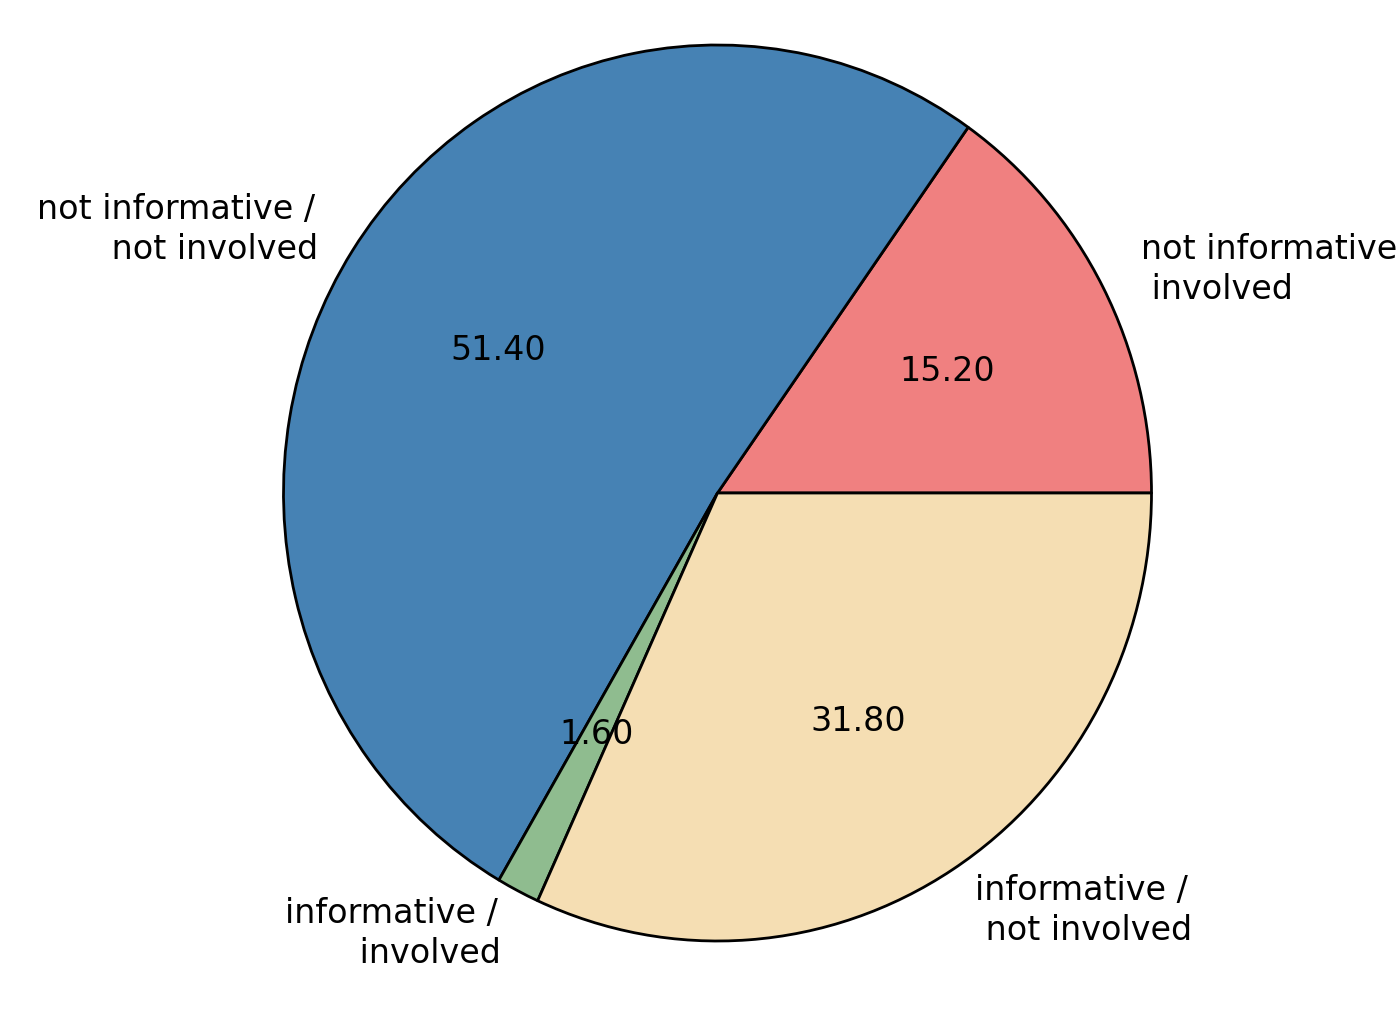
\includegraphics[width=\textwidth]{images/plots/pies/pie_pairs.png}
\end{subfigure}
\hfill
\begin{subfigure}[t]{0.42\textwidth}
\centering
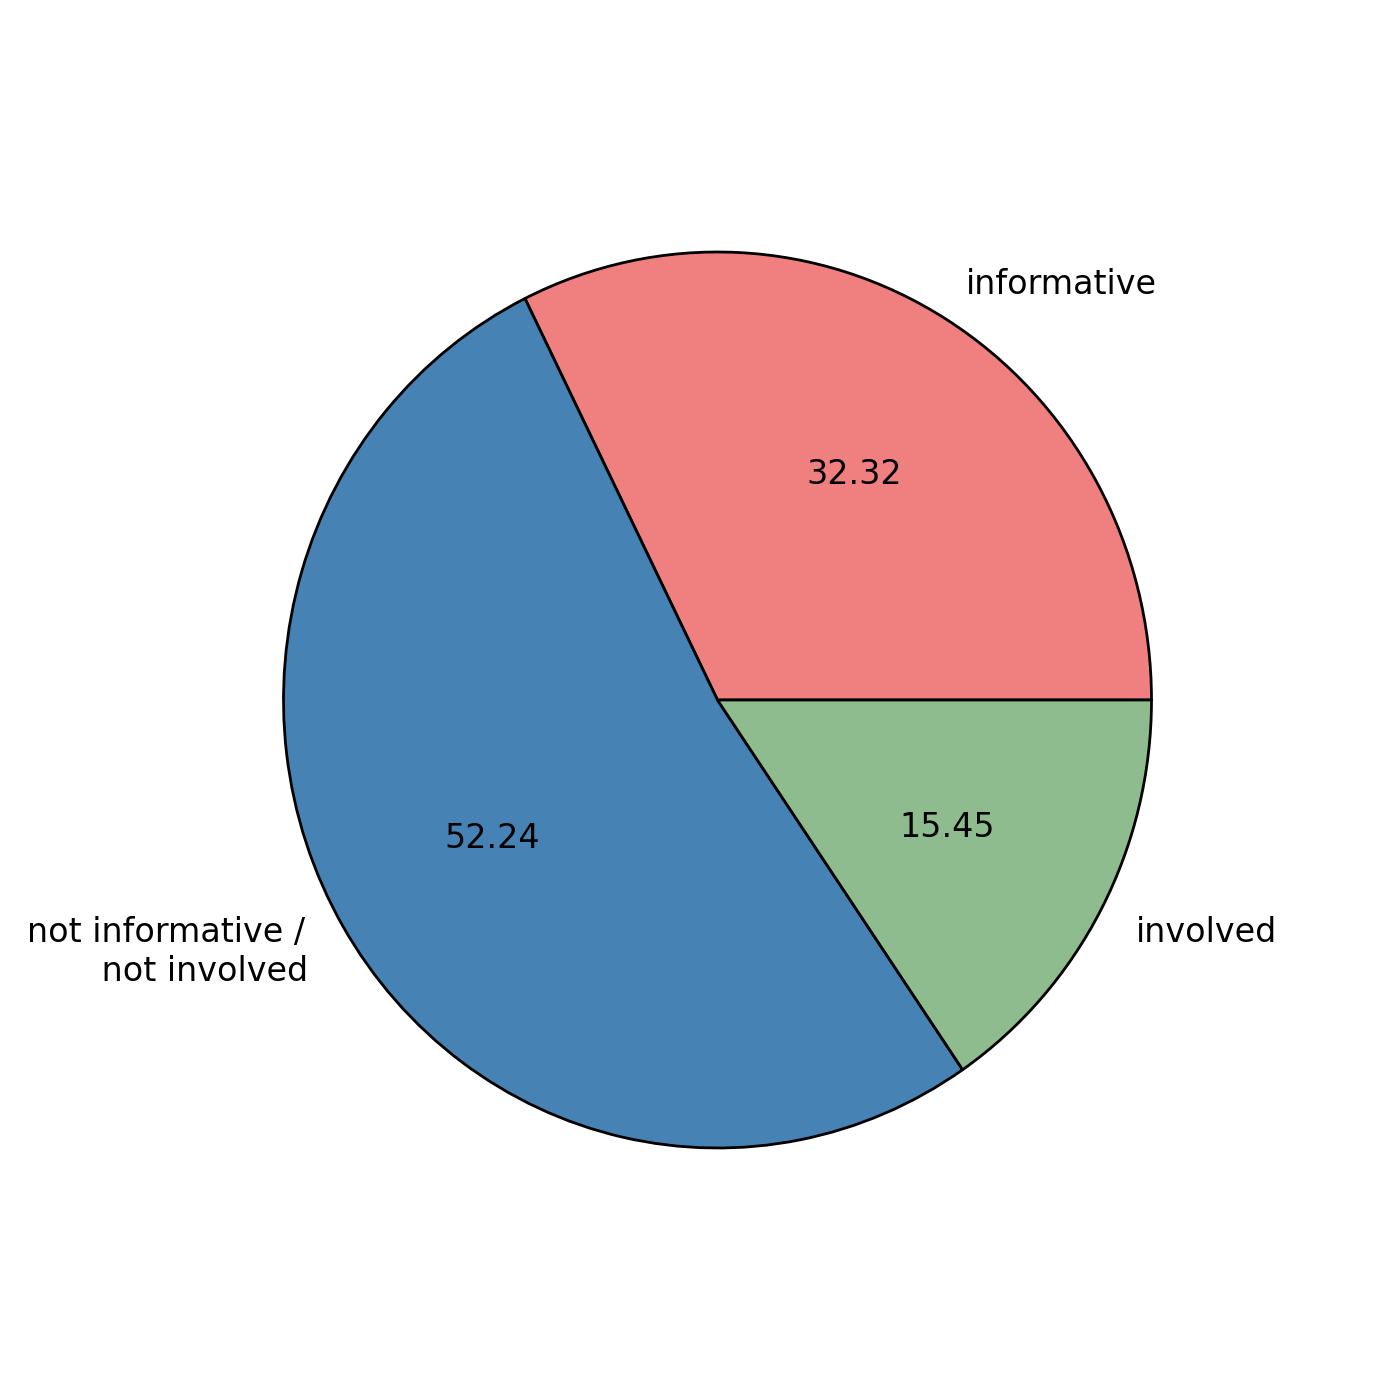
\includegraphics[width=\textwidth]{images/plots/pies/pie_pairs3.png}
\end{subfigure}
\end{figure}

\end{itemize}
\end{frame}

%%%%%%%%%%%%%%%%%%%%%%%%%%%%%%%%%%%%%%%%%%%%%%%%%%%%%%%%%%%%%%%%%%%%%%%%%%%%%%%%%%%%%%%%%%%%%

\begin{frame}{Model}
\begin{itemize}
\item Multinomial Naive Bayes
\begin{figure}[h!]
  \centering
\begin{tabular}{c|c|c|c|c||||c|}
\cline{2-6}
& class \# & 0 & 1 & 2 & \multirow{2}{*}{average}\\ \cline{2-5}
& meaning & $\neg$ i $\&$ $\neg$ s & i $\&$ $\neg$ s & $\neg$ i $\&$ s  & \\
\hline
\multicolumn{1}{|c|}{\multirow{2}{*}{\rotatebox{90}{NB}} } & unigrams & 84.9\% & 97.4\% & 85.9\% & 95.3\% \\
\multicolumn{1}{|c|}{} & bigrams & 80.4\% & 97.4\% & 78.5\% & 94.7\%   \\
\hline
\hline
\multicolumn{1}{|c|}{\multirow{2}{*}{\rotatebox{90}{PNB}}} & unigrams & 85.9\% & 97.6\% & 85.7\% & 95.6\%   \\
\multicolumn{1}{|c|}{} & bigrams & 83.2\% & 97.5\% & 79.9\% & 95.1\%   \\
\hline
\end{tabular}
\caption{F1 score on 5-fold cross-validation ; i = informative, s = supportive}
\end{figure}
\item 

\end{itemize}
\end{frame}

%%%%%%%%%%%%%%%%%%%%%%%%%%%%%%%%%%%%%%%%%%%%%%%%%%%%%%%%%%%%%%%%%%%%%%%%%%%%%%%%%%%%%%%%%%%%%

\begin{frame}{Model}
\begin{figure}[H]
\begin{subfigure}[t]{0.5\textwidth}
\begin{center}
	\includegraphics[width=\textwidth]{images/diags/media_features_1.png}
	\caption{class 1 (informative)}
	\label{impfeatureclass1}
\end{center}
\end{subfigure}
\begin{subfigure}[t]{0.42\textwidth}
\begin{center}
	\includegraphics[width=\textwidth]{images/diags/media_features_2.png}
	\caption{class 2 (supportive)}
	\label{impfeatureclass2}
\end{center}
\end{subfigure}
\caption{Most important features}
\end{figure}
\end{frame}

%%%%%%%%%%%%%%%%%%%%%%%%%%%%%%%%%%%%%%%%%%%%%%%%%%%%%%%%%%%%%%%%%%%%%%%%%%%%%%%%%%%%%%%%%%%%%

\section{Graph analysis and influence}
\begin{frame}{Outline}
\tableofcontents[sectionstyle=show/shaded]
\end{frame}

\begin{frame}{Hashtag graph}
\begin{itemize}
\item a \textbf{node} represents a hashtag
\item an \textbf{edge} between nodes $a$ and $b$ exists if $a$ and $b$ are used together is a tweet. Our edges are weighted such as the higher the weight, the more used hashtag combinaison.
\end{itemize}

\end{frame}

%%%%%%%%%%%%%%%%%%%%%%%%%%%%%%%%%%%%%%%%%%%%%%%%%%%%%%%%%%%%%%%%%%%%%%%%%%%%%%%%%%%%%%%%%%%%%

\begin{frame}{Hashtag graph}
\begin{figure}[H]
\centering
\includegraphics[width=0.7\textwidth]{images/graphs/hashtags/hc_13_08.png}
\label{graphHt13c}
\end{figure}
\end{frame}

%%%%%%%%%%%%%%%%%%%%%%%%%%%%%%%%%%%%%%%%%%%%%%%%%%%%%%%%%%%%%%%%%%%%%%%%%%%%%%%%%%%%%%%%%%%%%

\begin{frame}{Retweet graphs}
\begin{itemize}
\item a \textbf{node} represents a user
\item an \textbf{directed edge} from node $a$ to $b$ exists if $a$ retweets $b$. Our edges are weighted such as the higher the weight is, the more $a$ has retweeted $b$.
\end{itemize}
\end{frame}

%%%%%%%%%%%%%%%%%%%%%%%%%%%%%%%%%%%%%%%%%%%%%%%%%%%%%%%%%%%%%%%%%%%%%%%%%%%%%%%%%%%%%%%%%%%%%

\begin{frame}{Retweet graph}
\framesubtitle{August 17}
\begin{figure}[H]
\centering
\includegraphics[width=0.7\textwidth]{images/graphs/rtmentions/rtmentions_17.png}
\end{figure}
\end{frame}

%%%%%%%%%%%%%%%%%%%%%%%%%%%%%%%%%%%%%%%%%%%%%%%%%%%%%%%%%%%%%%%%%%%%%%%%%%%%%%%%%%%%%%%%%%%%%

\begin{frame}{Retweet graph}
\framesubtitle{August 17}
\begin{figure}[H]
\centering
\includegraphics[width=0.85\textwidth]{images/graphs/influence/gi_t0_1708.png}
\label{gi17}
\end{figure}
\end{frame}

%%%%%%%%%%%%%%%%%%%%%%%%%%%%%%%%%%%%%%%%%%%%%%%%%%%%%%%%%%%%%%%%%%%%%%%%%%%%%%%%%%%%%%%%%%%%%

\section{Role representation and visualization}
\begin{frame}{Outline}
\tableofcontents[sectionstyle=show/shaded]
\end{frame}

\begin{frame}{Unified model}
\begin{figure}[H]
\centering
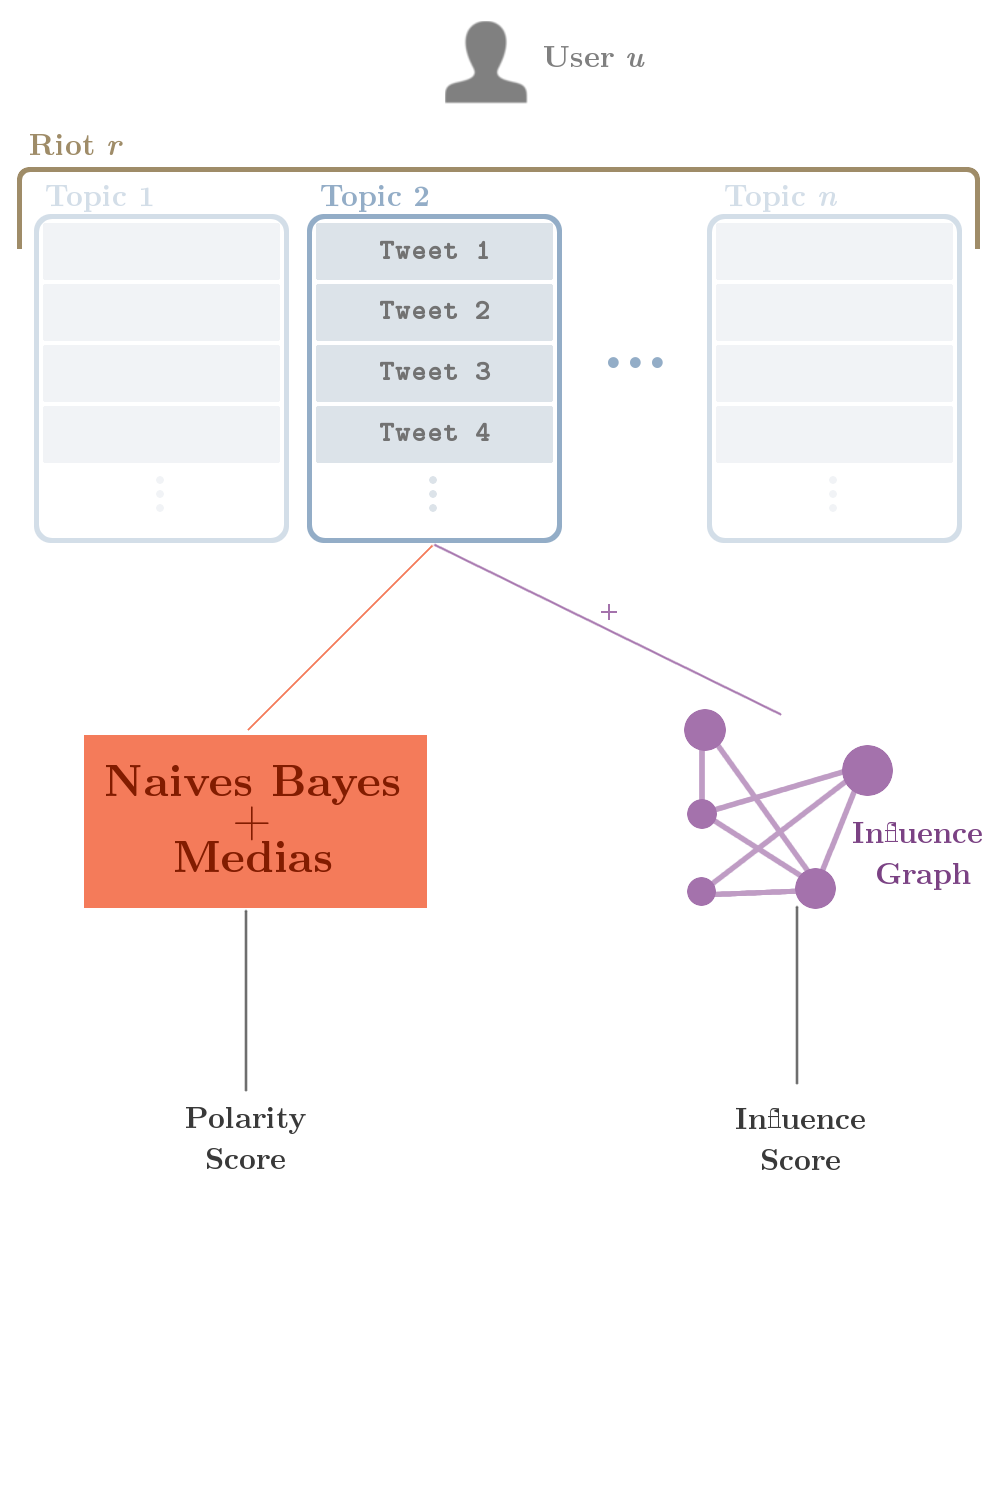
\includegraphics[width=0.5\textwidth]{images/diags/chain.png}
\ref{unifiedModel}
\end{figure}

\end{frame}

%%%%%%%%%%%%%%%%%%%%%%%%%%%%%%%%%%%%%%%%%%%%%%%%%%%%%%%%%%%%%%%%%%%%%%%%%%%%%%%%%%%%%%%%%%%%%

\begin{frame}{Unified model}
\begin{figure}[H]
\centering
\includegraphics[width=0.8\textwidth]{images/plots/roles/tsne_17_08.png}
\caption{$t$-SNE plot of the roles on the August 17th}
\label{}
\end{figure}
\end{frame}

%%%%%%%%%%%%%%%%%%%%%%%%%%%%%%%%%%%%%%%%%%%%%%%%%%%%%%%%%%%%%%%%%%%%%%%%%%%%%%%%%%%%%%%%%%%%%

\section{Conclusion}
\begin{frame}{Outline}
\tableofcontents[sectionstyle=show/shaded]
\end{frame}

\begin{frame}{Conclusions}
plop
\end{frame}

\end{document}
